\chapter{Software}
%%%%%%%%%%%%%%%%%%%%%%%%%%%%%%%%%%%%%%%%%%%%%%%%%%%%%%%%%%
Neste capitulo são apresentadas as ferramentas usadas no desenvolvimento do programa, e a estrutura do mesmo. Serão ainda apresentadas algumas explicações acerca do modo como o código foi implementado de forma ser atingido o objetivo proposto, que é o correto funcionamento da balança digital.
%%%%%%%%%%%%%%%%%%%%%%%%%%%%%%%%%%%%%%%%%%%%%%%%%%%%%%%%%%
\newpage
\section{Software}
O \ac{ide} utilizado neste trabalho foi o \textbf{\textit{{Microchip Studio for AVR\textsuperscript{\textregistered} and SAM Devices}}} (\textit{version: 7.0.2542}).
\emptyline
\begin{minipage}[!b]{.55\linewidth}
	\begin{figure}[H]
		\captionsetup{justification=raggedright,singlelinecheck=false}
		
\includegraphics[scale=0.55]{./image/PESTA/IDE/Microchip-Studio.png}
		\caption{Microchip Studio}
		\label{Microchip-Studio}
	\end{figure}
\end{minipage}
\begin{minipage}[!b]{.45\linewidth}
	Ao lado a \autoref{Microchip-Studio} mostra o logo da empresa, e abaixo a \autoref{Work-Space} apresenta o ambiente de trabalho onde é criado todo o código que vai correr no microcontrolador.
\emptyline
\end{minipage}
\minipagespace{.5}
\begin{figure}[H]
	\centering
	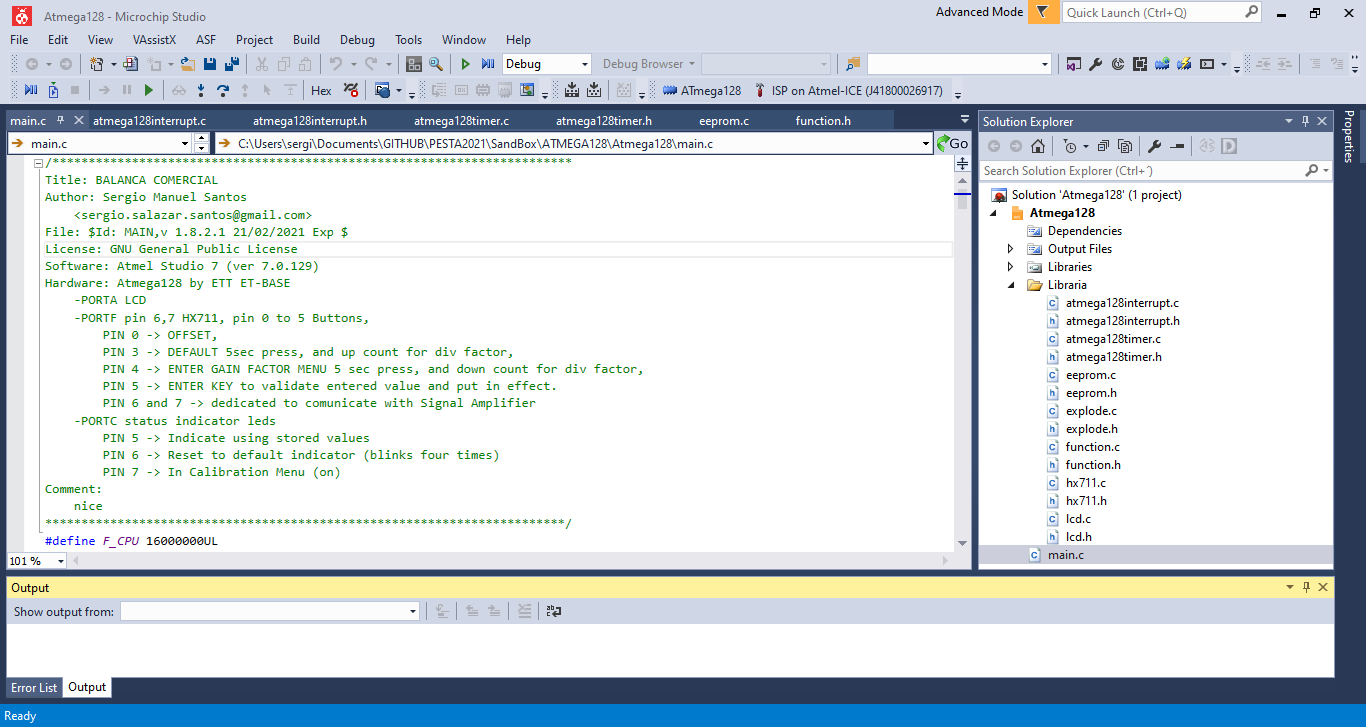
\includegraphics[width=\linewidth]{./image/PESTA/IDE/Work-Space.png}
	\caption{Ambiente de trabalho}
	\label{Work-Space}
\end{figure}
\figurespace{.5}
A programação foi feita em Linguagem \textbf{C} \cite{book-11}, e a sua estrutura sintática está abaixo apresentada na \autoref{Main_Program_1}:
\emptyline
%Mudar para Português
\begin{figure}[H]
	\centering
	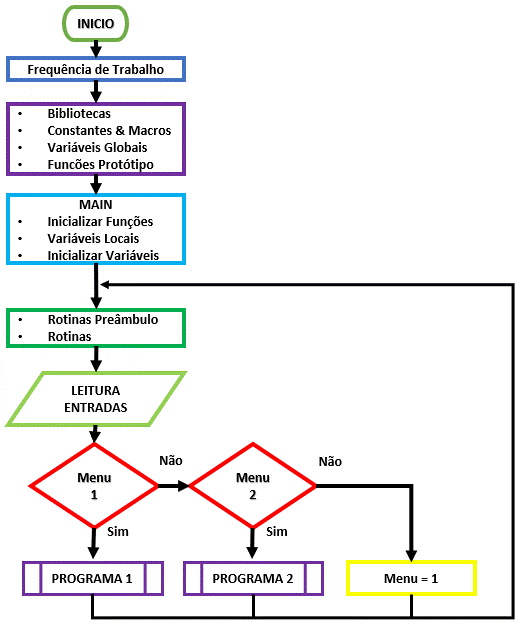
\includegraphics[scale=1]{./image/PESTA/flowchart/Main-Program-1.jpg}
	\caption{Estrutura do Programa}
	\label{Main_Program_1}
\end{figure}
\figurespace{.5}
O \textit{PROGRAMA 1} é onde corre o programa da balança, e o \textit{PROGRAMA 2} é usado para a calibração do fator de ganho.
\newpage
%O modelo de programação segue uma estrutura sintática de acordo com o seguinte modelo.
%\\
%\begin{figure}[H]
%	\centering
%	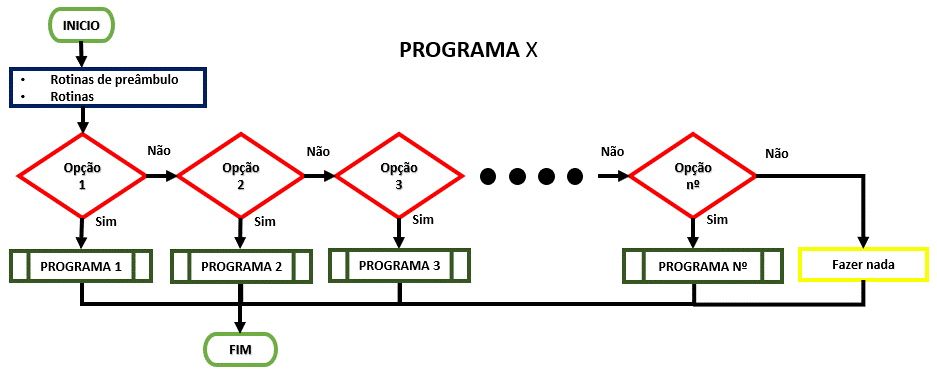
\includegraphics[height=8cm, width=\linewidth]{./image/PESTA/flowchart/Generic-structure-1.jpg}
%	\caption{Sintaxe genérica dos programas}
%	\label{Geneic_structure}
%\end{figure}
%\figurespace{.5}
Duas interrupções periódicas estão sempre a correr em \textit{background}, uma para fazer o \textit{shift} dos \textit{bits} da conversão \acs{adc} feita pelo amplificador de sinal HX711 e outra interrupção periódica de segundo em segundo, usada para saltar de \textit{Menu} pelos botões.
\\
\begin{minipage}{\linewidth}
	\begin{minipage}{.5\linewidth}
		\begin{figure}[H]
			\centering
			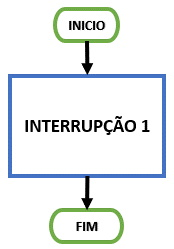
\includegraphics[scale=.85]{./image/PESTA/flowchart/Interrupt-1.jpg}
			\caption{\acs{adc} conversão}
			\label{Interrupt_1}
		\end{figure}
	\end{minipage}
	\begin{minipage}{.5\linewidth}
		\begin{figure}[H]
			\centering
			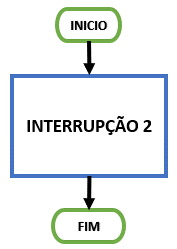
\includegraphics[scale=.85]{./image/PESTA/flowchart/Interrupt-2.jpg}
			\caption{Saltar de \textit{Menu}}
			\label{Interrupt_2}
		\end{figure}
	\end{minipage}
\end{minipage}
\minipagespace{.5}
%O código para leitura das rotinas de interrupção esta disponível nas folhas \textit{anexas} \ref{main-c}.
%É preferivel inseriri o excerto de código e descrever o funcionamento das interrupções
\begin{minipage}{.40\linewidth}
	\begin{figure}[H]
		\flushleft
		\captionsetup{justification=raggedright,singlelinecheck=false}
		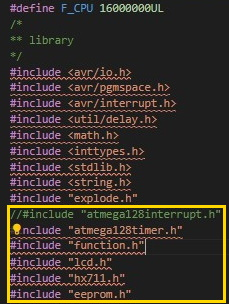
\includegraphics[scale=0.9]{./image/PESTA/Code/Livrarias.jpg}
		\caption{Bibliotecas}
		\label{Bibliotecas}
	\end{figure}
\end{minipage}
\hspace{2pt}
\begin{minipage}{.6\linewidth}
	Ao lado (\autoref{Bibliotecas}) estão as bibliotecas usadas neste projeto, as que estão dentro da caixa amarela são as que foram criadas pelo aluno.
	A filosofia usada é de criar objetos que representam o \textit{hardware} para o poder manipular via código. Como se pode observar, foi criada uma biblioteca para os temporizadores, outra para as interrupções e \ac{eeprom}, e por fim foram criadas bibliotecas para os componentes externos, isto é, o \acs{lcd} e o integrado \textbf{HX711}.\\
Uma abstração que torna simples executar qualquer algoritmo ou projeto, e isto só é possível depois de ultrapassar a barreira de desenvolver as bibliotecas.
\end{minipage}
\minipagespace{.3}
Durante este projeto foram seguidas as boas práticas de programação, como a da \texttt{indentação} específica para cada situação, e manter a estrutura de norma. Deve-se manter uma metodologia de trabalho que segue as normas, assim é percetível para qualquer programador e, não só evita bugs, mas também facilita a sua deteção. Esta é uma prática que abrange todas as linguagens.
%, por exemplo o \textbf{Python} é fundado nesse princípio.
\newpage
Quanto às interrupções é sempre um desafio, porque as tarefas têm que ser bem organizadas temporalmente para não entrar em conflitos, pretende-se assim que o código corra na função \textit{main} e as interrupções são algo esporádico e muito rápido, estas devem servir de \textit{flags} para executar rotinas na função \textit{main}, ou seja, servirem de \textit{inputs}. %%\textbf{\textcolor{green}{INPUTS}}.
%\newpage
%Passar isso para a parte de software
\emptyline
O código que executa a rotina de leitura \acs{adc} é apresentado na \autoref{HX711-read-raw}, sendo que esta é chamada pela interrupção periódica da \autoref{Interrupcao-1}, que só é ativa quando o resultado da função na \autoref{Main-While-case-1} \textbf{hx.query(\&hx)} é verdadeira.
\emptyline
{
	\lstinputlisting[language=C, caption={Interrupção 1}, captionpos=b, label=Interrupcao-1]{./input/code/Interrupcao-1.c}
}
\listingspace{.2}
{
	\lstinputlisting[language=C, caption={função de chamada \textbf{hx.query(\&hx)}}, captionpos=b, label=Main-While-case-1]{./input/code/hx_query.c}
}
\newpage
%Se apresenta código deve descreve-lo sucintamente
{
	\lstinputlisting[language=C, caption=HX711 read raw, captionpos=b, label=HX711-read-raw]{./input/code/HX711_read_raw.c}
}
Após obter um número determinado de valores discretos lidos pelo amplificador de célula de carga (HX711) é calculada uma média,
\begin{equation}
	\label{eq:Mean}
	\overline{x}  =  \frac{1}{n}\sum_{i=1}^n x_i
\end{equation}
para ser tratado e deduzido o valor correspondente do peso.
\newpage
O código da interrupção 2 está abaixo descrito na \autoref{Jump-menu} e serve para mudar de \textit{Menu} e limpar a \acs{eeprom}.
{
	\lstinputlisting[language=C, caption=Saltar de menu, captionpos=b, label=Jump-menu]{./input/code/Jump_menu.c}
}
%%%%%%%%%%%%%%%%%%%%%%%%%%%%%%%%%%%%%%%%%%%%%%%%%%%%%%%%%%
